\documentclass[pdf,azure,slideColor,colorBG]{prosper}

\usepackage[latin1]{inputenc}
\usepackage{pstricks,pst-node,pst-text,pst-3d}
\usepackage{amsmath}
\usepackage{graphics}
\usepackage{multicol}

\makeatletter
\define@key{PDF}{Movie}{\pdf@addtoks{#1}{Movie}}
\define@key{PDF}{Activation}{\pdf@addtoks{#1}{Activation}}
\newcommand{\moviewithpreview}[3]{% args: width, preview, movie
    \pdfmark[{\includegraphics[width=#1]{#2}}]{%
    pdfmark=/ANN,Subtype=/Movie,Movie=<< /F (#3) >>,%
    Activation=<< /ShowControls true /Mode /Repeat >>}}
\newcommand{\movie}[3]{% args:width, height, movie
    \pdfmark[{\hbox to #1 {\vbox to #2 { }}}]{%
    pdfmark=/ANN,Subtype=/Movie,Movie=<< /F (#3) /Poster true >>,%
    Activation=<< /ShowControls true /Mode /Repeat >>}}

% Args: width, preview, movie
\newcommand{\hrefWithPreview}[3]{%
  \href{#3}{\includegraphics[width=#1]{#2}}
}
%
\makeatother


\Logo{
\includegraphics[width=3cm]{nrc_newlogo.ps}}

\title{Simulating Focal Plane Array Observations with MeqTrees}
\author{\green Tony Willis} 
\email{tony.willis@nrc.ca}
\institution{ 
  National Research Council of Canada \\ Herzberg Institute of Astrophysics \\
  Penticton, BC, Canada V2A 6J9
}

\ptsize{10}
\begin{document}
\maketitle

\include{megi-symbols}
%---------------------------------------------------------------------- SLIDE -
\begin{slide}{Topics}
\begin{small}
\begin{itemize}
\item Overview of Measurement Equation
\item Overview of MeqTrees
\item Example of MeqTrees Configuration
\item Correction for E-Jones effects
\item Simulation Setup
\item Examples of MeqTrees Simulations
\begin{itemize}
\item Phase-Conjugate Weighting
\item Optimization for Gaussian beam shape
\item AzEl observation tracking a fixed offset position
\end{itemize}
\item What's Next?
\end{itemize}
\end{small}
\end{slide}
%------------------------------------------------------------------------------

%---------------------------------------------------------------------- SLIDE -
\begin{slide}{Measurement Equation - HBS}
{\centering
\resizebox*{0.6\columnwidth}{!}{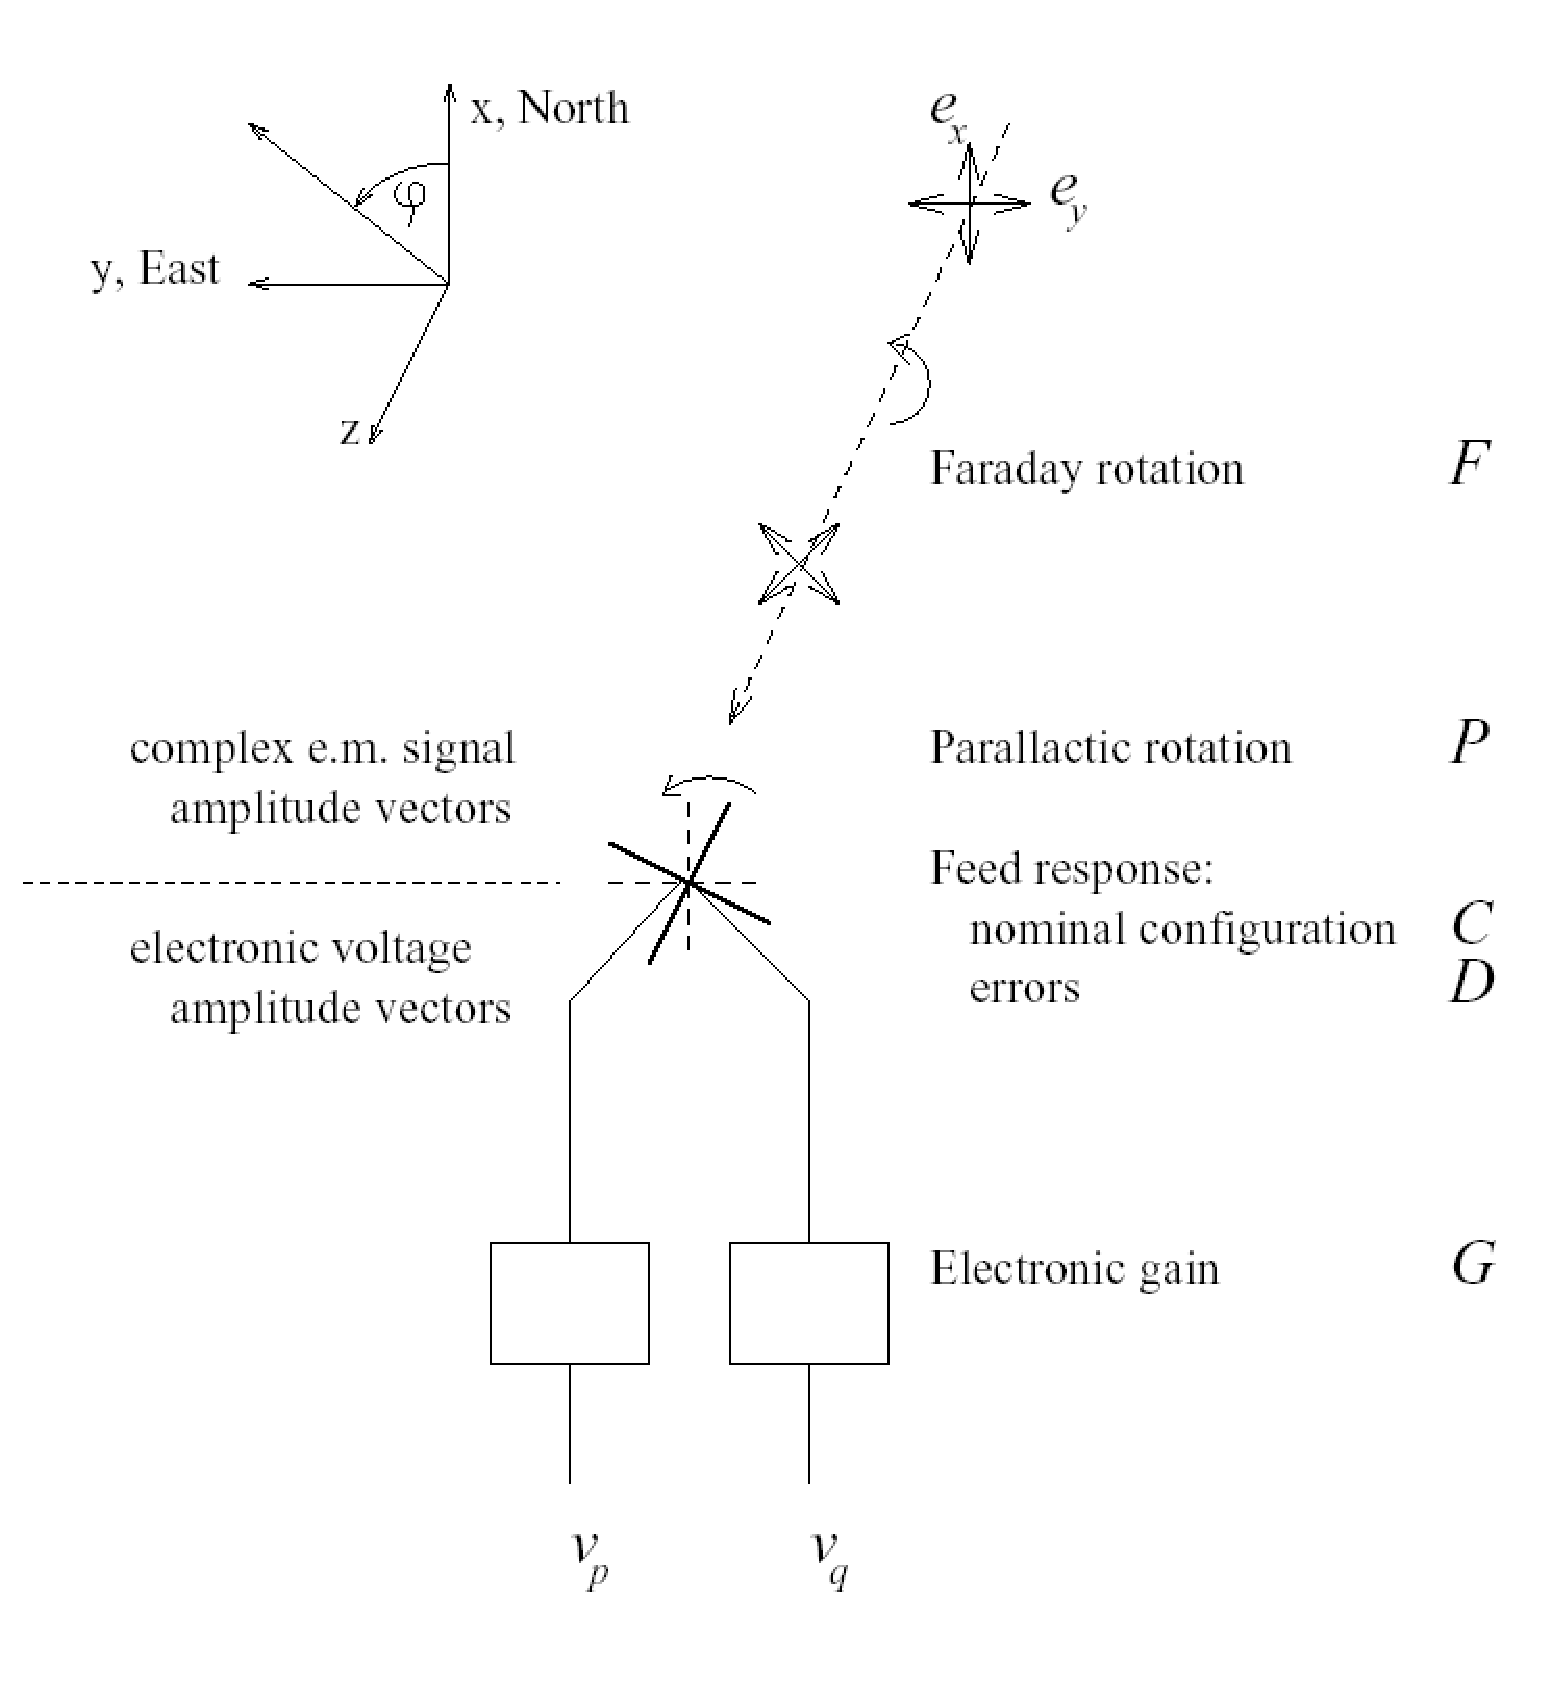
\includegraphics{schematic_transformations.ps}}
\par}
\end{slide}
%------------------------------------------------------------------------------

%---------------------------------------------------------------------- SLIDE -

\begin{slide}{Jones Matrices}
\begin{small}
\begin{itemize}
\item The real heart of the Measurement Equation (M.E.) is composed of
 of two $2\times2$ \Station-based response matrices, called `Jones matrices'.
\item The $2\times2$ Jones matrix $\mjJones\ssI$ for \Station\ $\StationI$ can
be decomposed into a product of several $2\times2$ Jones matrices,
each of which models a specific \Station-based instrumental effect in
the signal path (see Hamaker, Bregman, Sault papers and aips++ notes 
from Noordam and Cornwell).
\end{itemize}
\begin{displaymath}
  \mjJones\ssI 
  ~= 
  ~\mjGrec\ssI 
  ~[\mjHybr\ssI] 
  ~\mjBeam\ssI 
  ~\mjProj\ssI 
  ~\mjKern\ssI
  ~\mjTrop\ssI  
  ~\mjFrot\ssI 
  \label{eq:mjJones}
\end{displaymath}
\begin{itemize}
\item The visibility for an interferometer composed of
 \Station\ $\StationI$ and \Station\ $\StationJ$ with linearly polarized receptors is given by the following 
 equation, where $\vvCoh\ssIJ$ is the visibility, $~\vvIQUV$ is the 
 incoming electromagnetic coherency matrix,
 and $~\mjJones\ssJ^\ast$ is the complex conjugate of $\mjJones\ssJ$. 
\end{itemize}
\begin{displaymath}
  \vvCoh\ssIJ 
  ~= 
  ~\mjJones\ssI 
  ~\vvIQUV
  ~\mjJones\ssJ^\ast
  \label{eq:mjJones}
\end{displaymath}
\begin{displaymath}
  \vvIQUV
  ~=
  ~0.5
  ~\tbt {I+Q}  {U-iV}
        {U+iV}  {I-Q}
\end{displaymath}
\end{small}
\end{slide}                             

%---------------------------------------------------------------------- SLIDE -

\begin{slide}{Jones Matrix Definitions}
\vspace{-0.5cm}	
\begin{small}
\begin{tabbing}
++++\=++++++\= \kill   %tabs
\+					% start at 1st tab
~\\ $\mjFrot\ssI(\vvLMN,\vvAntPos\ssI)$   \> ionospheric Faraday rotation 
~\\ $\mjTrop\ssI(\vvLMN,\vvAntPos\ssI)$   \> atmospheric complex gain
~\\ $\mjKern\ssI(\vvLMN.\vvAntPos\ssI)$   \> factored Fourier Transform kernel 
~\\ $\mjProj\ssI$     \> projected \Receptor\ orientation(s) w.r.t. the sky
%%~\\ $\mjBeam\ssI(\vvLMN)$                 \> voltage primary beam
~\\ $\mjBeam\ssI(\vvLMN,\vvAntPos\ssI)$     \> voltage primary beam
~\\ $[\mjHybr\ssI]$     \> hybrid (conversion to circular polarization
                         coord)
~\\ $\mjGrec\ssI$     \> electronic complex gain (\Station\ contributions)
\end{tabbing}


\begin{itemize}
\item E-Jones definition
\begin{displaymath}
 \mjBeam\ssLI(\vvLMN,\vvAntPos\ssI)
  ~=
  ~\mjBeam\ssCI(\vvLMN,\vvAntPos\ssI)
  ~=
  ~\mjBeam\ssI(\vvLMN,\vvAntPos\ssI)
  ~=
  \tbt {\mjBeamEl\ssIAA}   {\mjBeamEl\ssIBA}
       {\mjBeamEl\ssIAB}   {\mjBeamEl\ssIBB}
\end{displaymath}
\item On axis diagonal terms describe position dependant primary beam attenuation
\item Non-zero off-diagonal terms $\mjBeamEl\ssIBA$ and $\mjBeamEl\ssIAB$ describe `leakage' between \Receptors
\end{itemize}
\end{small}
\end{slide}                             
%---------------------------------------------------------------------- SLIDE -

%---------------------------------------------------------------------- SLIDE -
\begin{slide}{MeqTrees Summary}
\begin{small}
\begin{itemize}
\item M.E. predicts data measured with a particular instrument.
\begin{itemize}
\item Model the instrument and observed data
\item Use for both system calibration and extraction of data parameters
\item Work mostly with Fourier (Visibility) data
\end{itemize}
\item Procedure
\begin{itemize}
\item Implement model in software using tree structure
\item Use a priori guesses to set model parameters
\item Compare observed data with predicted values
\item Solver/Condeq nodes adjust model parameters for best fit
\item Can solve for many discrepant parameters at same time 
\begin{itemize}
\item Hubble constant not yet done
\end{itemize}
\end{itemize}
\item Multi-threaded processing available
\item In on-going development
\item NOT an antenna / FPA design tool or a synthesis imaging tool
\end{itemize}
\end{small}
\end{slide}
%-----------------------------------------------------------------------

%---------------------------------------------------------------------- SLIDE -

\begin{slide}{Example E-Jones Calculation}
\begin{small}
\begin{itemize}
\item The voltage beam pattern, E, of a Large Aperture Reflector (LAR)
 measured at the position of a source
 whose direction coordinates L and M are defined with respect to the field 
 centre in an AzEl reference frame can be given as:
\end{itemize}
\begin{displaymath}
\rm E(L,M) = \sqrt{exp(-\ln16 \times (\frac{1}{\rm HPBW})^2(\rm L^2 + (        M \sin(\rm El))^2))}
\end{displaymath}
\begin{itemize}
\item HPBW $=$ half power beam width at zenith
\item El $=$ elevation of field or tracking centre
\end{itemize}
\end{small}
\end{slide}
%---------------------------------------------------------------------- SLIDE -

%---------------------------------------------------------------------- SLIDE -
\begin{slide}{The LAR Beam as a MeqTree}
{\centering
\resizebox*{0.5\columnwidth}{!}{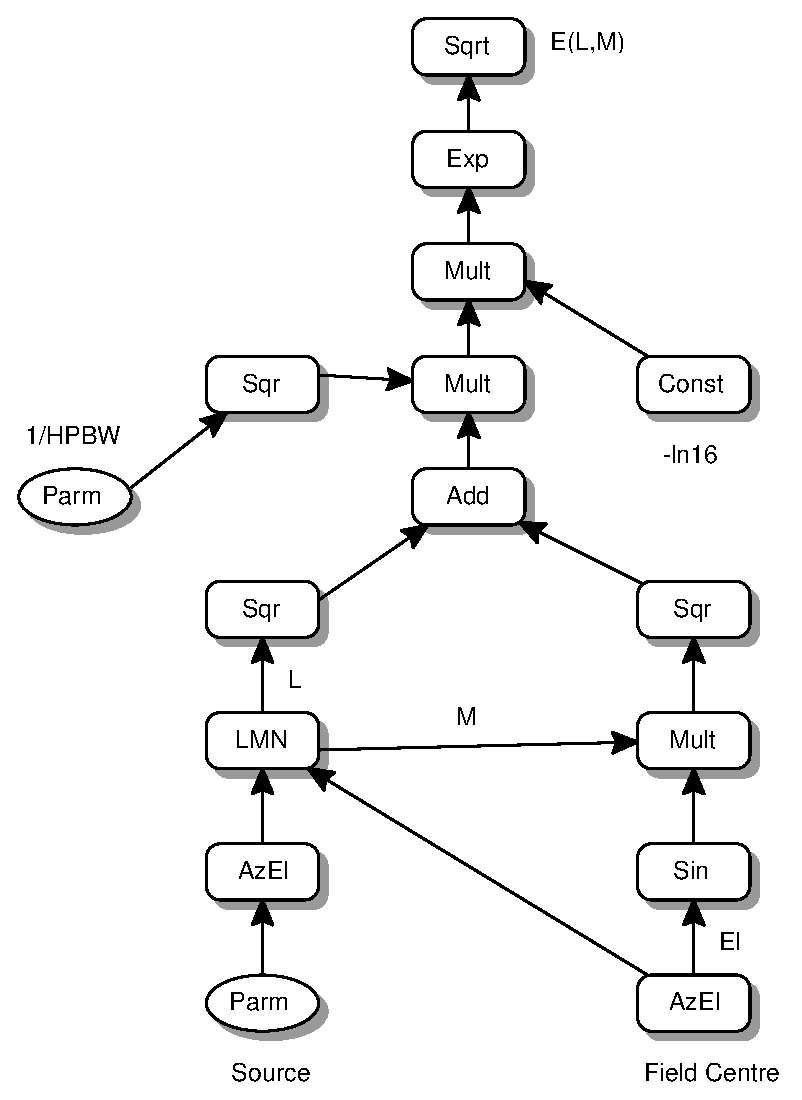
\includegraphics{LAR_MeqTree.eps}}
\par}
\end{slide}
%---------------------------------------------------------------------- SLIDE -

%---------------------------------------------------------------------- SLIDE -
\begin{slide}{Reduction Goals}
\begin{small}
\begin{itemize}
\item Left - most reduction packages; Right - MeqTrees
\end{itemize}
\end{small}
{\centering
\resizebox*{0.27\columnwidth}{!}{\includegraphics{3C449.ps}}
\resizebox*{0.27\columnwidth}{!}{\includegraphics{3C449_background.ps}}
\par}
\end{slide}
%---------------------------------------------------------------------------

%---------------------------------------------------------------------- SLIDE -
\begin{slide}{Know Thy E-Jones}
\begin{small}
\begin{itemize}
\item No longer acceptable to model primary beams as simple Gaussians
\item South Africa SKA Calibration and Imaging Workshop 2006 
\begin{itemize}
\item At least 4 or 5 presentations concerned with detailed measurements of telescope primary beams
\item Example - work of R. Reid et al. at DRAO on polarization leakage
\begin{itemize}
\item Each telescope of DRAO SST has different E-Jones voltage pattern
\item Detailed measurements made of the pattern for each dish
\item Accurate correction for instrumental polarization now possible   
\end{itemize}
\end{itemize}
\end{itemize}
\end {small}
\end{slide}
%------------------------------------------------------------------------------

%---------------------------------------------------------------------- SLIDE -
\begin{slide}{DRAO Stokes I}
{\centering
\resizebox*{0.6\columnwidth}{!}{\includegraphics{stokes_I.ps}}
\par}
\end{slide}
%------------------------------------------------------------------------------

%---------------------------------------------------------------------- SLIDE -
\begin{slide}{Stokes U No Correction}
{\centering
\resizebox*{0.6\columnwidth}{!}{\includegraphics{stokes_two.ps}}
\par}
\end{slide}
%------------------------------------------------------------------------------

%---------------------------------------------------------------------- SLIDE -
\begin{slide}{Stokes U Corrected}
{\centering
\resizebox*{0.6\columnwidth}{!}{\includegraphics{stokes_one.ps}}
\par}
\end{slide}
%------------------------------------------------------------------------------

%---------------------------------------------------------------------- SLIDE -
\begin{slide}{Know Thy FPA E-Jones}
\begin{small}
\begin{itemize}
\item Detailed knowledge of individual FPA voltage patterns allows
accurate `first order' prediction of phased array beam shapes
\begin{itemize}
\item Resampling and interpolation tools allow extrapolation from 
coarse `grid' measurements of actual FPA elements to finer grid for 
prediction of actual values associated with radio sources in the field
\end{itemize}
\item Assuming MIRANdA / SKA dishes and receiver elements are stamped out of 
uniform molds, detailed measurements of FPA voltage patterns on 
`representative' dishes should allow us to model entire array.
\item GRASP calculations are the equivalent of the above activity for
purposes of the simulations presented here.
\end{itemize}
\end {small}
\end{slide}
%------------------------------------------------------------------------------


%---------------------------------------------------------------------- SLIDE -
\begin{slide}{Simulated FPA}
\begin{small}
\begin{itemize}
\item 30 dipole elements in each of X and Y directions
\item Frequency = 1500 MHz; Spacing = lambda / 2
\item Dish diameter = 10m; Focal length = 4.5m
\item No coupling between elements; No feed struts in simulation
\item Not meant as a `realistic' final FPA design, but a good
testbed for various aspects of software development and data processing
\end{itemize}
\end {small}
{\centering
\resizebox*{0.4\columnwidth}{!}{\includegraphics{dipole_array_layout.ps}}
\par}
\end{slide}
%------------------------------------------------------------------------------

%---------------------------------------------------------------------- SLIDE -
\begin{slide}{Simulation Procedure}
\begin{small}
\begin{itemize}
\item Do GRASP calculations of voltage radiation patterns for each of the 
X and Y dipoles used in this simulation
\begin {itemize}
\item We get both co-polarization and cross-polarization leakage terms
\end{itemize}
\item Convert GRASP `grd' files to FITS images
\item MeqTrees reads in radiation patterns from the FITS images
\item Phase up X and Y radiation patterns, depending on optimization criteria,
for requested observing position. In most of the simulations shown here 
we observe on a 5 x 5 grid centred on L=M=0, in steps of 82 arcmin (HPBW). 
\item Form E-Jones Matrix (fully complex) from weighted combinations
\item Simulate observations of the `visible' sky via our equation:
\end{itemize}
\begin{displaymath}
  \vvCoh\ssIJ 
  ~= 
  ~\mjBeam\ssI
  ~\vvIQUV
  ~\mjBeam\ssJ^\ast
\end{displaymath}
\end {small}
\end{slide}
%------------------------------------------------------------------------------

%---------------------------------------------------------------------- SLIDE -
\begin{slide}{Typical GRASP Dipole Pattern}
\begin{small}
\begin{itemize}
\item In reality, we must measure these patterns in order to do accurate 
predicts, and thus compare with observations
\end{itemize}
\end {small}
{\centering
\resizebox*{0.65\columnwidth}{!}{\includegraphics{Voltage_pat1.ps}}
\par}
\end{slide}
%------------------------------------------------------------------------------

%---------------------------------------------------------------------- SLIDE -
\begin{slide}{Sky Coverage}
\begin{small}
\begin{itemize}
\item Basically we can attempt to do beam-forming over the range -0.05 to 0.05 radians in L and M.
\end{itemize}
\end {small}
{\centering
\resizebox*{0.6\columnwidth}{!}{\includegraphics{sky_coverage_linear.ps}}
\par}
\end{slide}                             
%---------------------------------------------------------------------- SLIDE -

%---------------------------------------------------------------------- SLIDE -
\begin{slide}{Phase Conjugate Weighting - I}
\begin{small}
\begin{itemize}
\item Phase conjugate weighting maximizes gain in observed
direction, but does nothing particular for beam shape
\item demo shows I beams for central row as we move from left edge toward centre of array in steps of 82 arcmin (HPBW)
\end{itemize}
\end {small}
{\centering
\resizebox*{0.3\columnwidth}{!}{\includegraphics{I_11.ps}}
\resizebox*{0.3\columnwidth}{!}{\includegraphics{I_12.ps}}
\resizebox*{0.3\columnwidth}{!}{\includegraphics{I_13.ps}}
\par}
\end{slide}

%---------------------------------------------------------------------- SLIDE -

%---------------------------------------------------------------------- SLIDE -
\begin{slide}{Phase Conjugate Weighting - I}
\begin{small}
\begin{itemize}
\item Phase conjugate weighting maximizes gain in observed
direction, but does nothing particular for beam shape
\item demo shows I beams for middle row as we move from left edge toward centre of array in steps of 82 arcmin (HPBW)
\end{itemize}
\end {small}
{\centering
\resizebox*{0.3\columnwidth}{!}{\includegraphics{I_16.ps}}
\resizebox*{0.3\columnwidth}{!}{\includegraphics{I_17.ps}}
\resizebox*{0.3\columnwidth}{!}{\includegraphics{I_18.ps}}
\par}
\end{slide}

%---------------------------------------------------------------------- SLIDE -

%---------------------------------------------------------------------- SLIDE -
\begin{slide}{Phase Conjugate Weighting - I}
\begin{small}
\begin{itemize}
\item Phase conjugate weighting maximizes gain in observed
direction, but does nothing particular for beam shape
\item demo shows I beams as we move along top edge of array in steps of 82 arcmin (HPBW)
\end{itemize}
\end {small}
{\centering
\resizebox*{0.3\columnwidth}{!}{\includegraphics{I_21.ps}}
\resizebox*{0.3\columnwidth}{!}{\includegraphics{I_22.ps}}
\resizebox*{0.3\columnwidth}{!}{\includegraphics{I_23.ps}}
\par}
\end{slide}
%---------------------------------------------------------------------- SLIDE -

%---------------------------------------------------------------------- SLIDE -
\begin{slide}{Phase Conjugate Weighting - Q}
\begin{small}
\begin{itemize}
\item demo shows Q response for central row as we move from left edge toward centre of array in steps of 82 arcmin (HPBW)
\end{itemize}
\end {small}
{\centering
\resizebox*{0.3\columnwidth}{!}{\includegraphics{Q_11.ps}}
\resizebox*{0.3\columnwidth}{!}{\includegraphics{Q_12.ps}}
\resizebox*{0.3\columnwidth}{!}{\includegraphics{Q_13.ps}}
\par}
\end{slide}

%---------------------------------------------------------------------- SLIDE -

%---------------------------------------------------------------------- SLIDE -
\begin{slide}{Phase Conjugate Weighting - Q}
\begin{small}
\begin{itemize}
\item demo shows Q response for middle row as we move from left edge toward centre of array in steps of 82 arcmin (HPBW)
\end{itemize}
\end {small}
{\centering
\resizebox*{0.3\columnwidth}{!}{\includegraphics{Q_16.ps}}
\resizebox*{0.3\columnwidth}{!}{\includegraphics{Q_17.ps}}
\resizebox*{0.3\columnwidth}{!}{\includegraphics{Q_18.ps}}
\par}
\end{slide}

%---------------------------------------------------------------------- SLIDE -

%---------------------------------------------------------------------- SLIDE -
\begin{slide}{Phase Conjugate Weighting - Q}
\begin{small}
\begin{itemize}
\item demo shows Q response as we move along top edge of array in steps of 82 arcmin (HPBW)
\end{itemize}
\end {small}
{\centering
\resizebox*{0.3\columnwidth}{!}{\includegraphics{Q_21.ps}}
\resizebox*{0.3\columnwidth}{!}{\includegraphics{Q_22.ps}}
\resizebox*{0.3\columnwidth}{!}{\includegraphics{Q_23.ps}}
\par}
\end{slide}
%---------------------------------------------------------------------- SLIDE -

%---------------------------------------------------------------------- SLIDE -
\begin{slide}{Optimized Gaussian Beam - I}
\begin{small}
\begin{itemize}
\item Obtain values for phase-conjugate weighting in a particular direction
\item Provide these values as initial guess for weights to MeqTrees solver
\item Solver adjusts weights until phased beam has optimal gaussian shape
\item demo shows I beams for central row as we move from left edge toward centre of array in steps of 82 arcmin (HPBW)
\end{itemize}
\end {small}
{\centering
\resizebox*{0.3\columnwidth}{!}{\includegraphics{I_gauss_11.ps}}
\resizebox*{0.3\columnwidth}{!}{\includegraphics{I_gauss_12.ps}}
\resizebox*{0.3\columnwidth}{!}{\includegraphics{I_gauss_13.ps}}
\par}
\end{slide}

%---------------------------------------------------------------------- SLIDE -

%---------------------------------------------------------------------- SLIDE -
\begin{slide}{Optimized Gaussian Beam - I}
\begin{small}
\begin{itemize}
\item Obtain values for phase-conjugate weighting in a particular direction
\item Provide these values as initial guess for weights to MeqTrees solver
\item Solver adjusts weights until phased beam has optimal gaussian shape
\item demo shows I beams for middle row as we move from left edge toward centre of array in steps of 82 arcmin (HPBW)
\end{itemize}
\end {small}
{\centering
\resizebox*{0.3\columnwidth}{!}{\includegraphics{I_gauss_16.ps}}
\resizebox*{0.3\columnwidth}{!}{\includegraphics{I_gauss_17.ps}}
\resizebox*{0.3\columnwidth}{!}{\includegraphics{I_gauss_18.ps}}
\par}
\end{slide}

%---------------------------------------------------------------------- SLIDE -
%---------------------------------------------------------------------- SLIDE -
\begin{slide}{Optimized Gaussian Beam - I}
\begin{small}
\begin{itemize}
\item Obtain values for phase-conjugate weighting in a particular direction
\item Provide these values as initial guess for weights to MeqTrees solver
\item Solver adjusts weights until phased beam has optimal gaussian shape
\item demo shows I beams as we move along top edge of array in steps of 82 arcmin (HPBW)
\end{itemize}
\end {small}
{\centering
\resizebox*{0.3\columnwidth}{!}{\includegraphics{I_gauss_21.ps}}
\resizebox*{0.3\columnwidth}{!}{\includegraphics{I_gauss_22.ps}}
\resizebox*{0.3\columnwidth}{!}{\includegraphics{I_gauss_23.ps}}
\par}
\end{slide}

%---------------------------------------------------------------------- SLIDE -

%---------------------------------------------------------------------- SLIDE -
\begin{slide} {AzEl Telescope Simulation - I}
\begin{small}
\begin{itemize}
\item Calculate Parallactic Angle as a function of time for AzEl-mounted
telescope stationed at VLA site which tracks position RA = 0 hr, Dec = 0 deg
\item Phase up FPA at a position whose offset with respect to the
tracking centre is -0.02 radians in both L and M when the Parallactic Angle is zero (transit)
\item Adjust FPA phase conjugate weights to keep beam centred on this
position.
\begin{itemize}
\item 8 hour observation; calculate FPA beam every 10 minutes
\end{itemize}
\item Total Intensity beam shown for start, middle and end of observation 
\end{itemize}
\end {small}
{\centering
\resizebox*{0.3\columnwidth}{!}{\includegraphics{I_azel_1.ps}}
\resizebox*{0.3\columnwidth}{!}{\includegraphics{I_azel_24.ps}}
\resizebox*{0.3\columnwidth}{!}{\includegraphics{I_azel_48.ps}}
\par}
\end{slide}

%---------------------------------------------------------------------- SLIDE -

%---------------------------------------------------------------------- SLIDE -
\begin{slide} {AzEl Telescope Simulation - Q}
\begin{small}
\begin{itemize}
\item Calculate Parallactic Angle as a function of time for AzEl-mounted
telescope stationed at VLA site which tracks position RA = 0 hr, Dec = 0 deg
\item Phase up FPA at a position whose offset with respect to the
tracking centre is -0.02 radians in both L and M when the Parallactic Angle is zero (transit)
\item Adjust FPA phase conjugate weights to keep beam centred on this
position.
\begin{itemize}
\item 8 hour observation; calculate FPA beam every 10 minutes
\end{itemize}
\item Q response shown for start, middle and end of observation 
\end{itemize}
\end {small}
{\centering
\resizebox*{0.3\columnwidth}{!}{\includegraphics{Q_azel_1.ps}}
\resizebox*{0.3\columnwidth}{!}{\includegraphics{Q_azel_24.ps}}
\resizebox*{0.3\columnwidth}{!}{\includegraphics{Q_azel_48.ps}}
\par}
\end{slide}

%---------------------------------------------------------------------- SLIDE -

%---------------------------------------------------------------------- SLIDE -
\begin{slide}{Modcal - Remove Anything}
\begin{itemize}
\item Algorithm developed at DRAO to get rid of unwanted sources when you don't have a good understanding of your E-Jones.
\item Baseline-based rather than antenna-based so not really part of the Jones Matrix formalism.
\item Can be useful as a method of last resort.
\item Only about 20 lines of python code with MeqTrees.
\end{itemize}
\end{slide}
%------------------------------------------------------------------------------

%---------------------------------------------------------------------- SLIDE -
\begin{slide}{Modcal - Example}
\begin{small}
\begin{itemize}
\item Right image shows source in sidelobe which does not clean properly; left image shows source vaporised by modcal algorithm.
\end{itemize}
\end {small}
{\centering
\resizebox*{0.9\columnwidth}{!}{\includegraphics{modcal_demo.ps}}
\par}
\end{slide}
%------------------------------------------------------------------------------


%---------------------------------------------------------------------- SLIDE -
\begin{slide}{Conclusion: Know Thy E-Jones}
\begin{itemize}
\item Heuristics
\item Learning
\end{itemize}
\end{slide}
%------------------------------------------------------------------------------
%---------------------------------------------------------------------- SLIDE -
\begin{slide}{What's Next?}
\ptsize{10}
\begin{itemize}
\item Need Better Optimization than Gaussian Beam
\begin{itemize}
\item Spheroids
\item Kaiser-Bessel
\end{itemize}
\item Generate GRASP models of antennas more suitable for FPA such
as Vivaldis and simulate observations with them.
\item Look at effects of system gain variations on formed beams.
\end{itemize}
`Solving for the Hubble constant (say as a polc in time) should be
possible too, but you need a machine big enough to model the universe
on....'

- Oleg M Smirnov, Russian/Dutch computer scientist
\end{slide}
%---------------------------------------------------------------------- SLIDE -

%---------------------------------------------------------------------- SLIDE -
\begin{slide}{Questions?}
\begin{itemize}
\item Email: tony.willis@nrc.ca
\end{itemize}
\end{slide}                             
%---------------------------------------------------------------------- SLIDE -

%---------------------------------------------------------------------- SLIDE -
\begin{slide}{Acknowledgements}

\begin{small}
\begin{itemize}
\item MeqTrees team, especially Oleg Smirnov, Maaijke Mevius and Sarod Yatawatta for assistance on MeqProblems related to focal plane arrays
\item Jan Noordam for aips++ Note 185 on the Measurement Equation
\item Bruce Veidt for GRASP calculations and advice on antenna-related issues
\item 3C449 image made (a long time ago) at the VLA, operated by NRAO / AUI / NSF
\end{itemize}
\end{small}
\end{slide}
%---------------------------------------------------------------------- SLIDE -
\end{document}


\end{document}

